\section{Overview}
\label{section:overview}
In this work, we propose to steer high-dimensional data exploration via local data analysis. Our approach facilitates local analysis in an efficient and distortion-free way. In this section, we first clarify the concept of local distortion reduction. Then we demonstrate how it can be used to guide the high-dimensional exploration. At last, we give an overview of the interactive exploration process supported by our method.

\subsection{Local Distortion Reduction}
Reducing local projection distortion is a major goal in this work. However, our definition of distortion is more than mere projection errors. Traditionally, distortion refers to the gap between original data distances and the projected distances. We call it the \emph{distance distortion}. Efforts paid to reduce such distortion globally, results in various kinds of dimension reduction techniques~\cite{jolliffe2002principal}~\cite{borg2005modern}~\cite{tenenbaum2000global}~\cite{roweis2000nonlinear}. But a more recent research~\cite{DBLP:journals/tvcg/EtemadpourMPMOL15} has shown that, those projections cannot guarantee a good performance for certain analytic tasks. The main cause, in our opinion, is the existence of relationship distortions.

By 'relationship', we refer to a relative concept of distance, i.e. 'close' or 'far'. In the high-dimensional space, relationship should be defined based on data range and the dimensional subspace. Assume that there are four data items distributed in a two-dimensional plane, as shown in Figure 2. When talking about data A, B and C, we can say that 'C is far away from B (compared to A)'. But when talking about data B, C and D, C seems close to B (compared to D). On the other hand, C is closer to B than A in dimension X, while the opposite happens in dimension Y. When combing all data and dimensions, weaker relationships give way to the stronger ones. The weak ones (e.g. C is closer to B than A) can no longer be perceived. Even the strong ones are not as obvious as in the original context. We call it the \emph{relationship distortion}. The situation is alike in more complex real-world datasets. In summary, integrated distances cannot reflect local relationships precisely. That's why reducing distance distortion cannot guarantee more featured relationships.

Our approach aims to reduce both kinds of distortions, especially the relationship distortion. It is the key to revealing hidden local features. Specifically, we allow users to focus on a data subset to accommodate relationships in different ranges. In addition, projection pursuit is applied to enhance relationships in different subspaces. More details will be introduced in Section~\ref{section:method}.

\subsection{High-dimensional Exploration Guided by Local Data Analysis}

To be specific, the exploration contains four steps:
\begin{enumerate}[(1)]
 \item First, for any given projection, we help the user find a piece of interesting local data. Projection distortion and cluster suggestions are displayed to indicate potential outliers and clusters. The data chosen by user is called a 'focus', meaning that it's the current focus in local analysis.
 \item After some focus is chosen, we find its most featured projections for a targeted analysis. By 'features', we refer to three kinds of relationships we defined based on data distances. Projections are optimized to show these features with the least distortion.
 \item Since the focus is chosen in a projection, it could be a false cluster or missing some important pieces. We provide suggestions to help shape the focus into a more consistent and complete cluster. Whenever the focus is changed, the feature projections will also be updated.
 \item When some informative local data is found, the user can store it in a focus list. A 'projection map' is provided for all feature projections. It helps to compare different focuses, and navigate the high-dimensional exploration.
\end{enumerate}
 With our method, users are able to explore the data space efficiently, by analyzing different parts of local data in a distortion-free way.

\ifx
\begin{figure*}[htb]
\centering
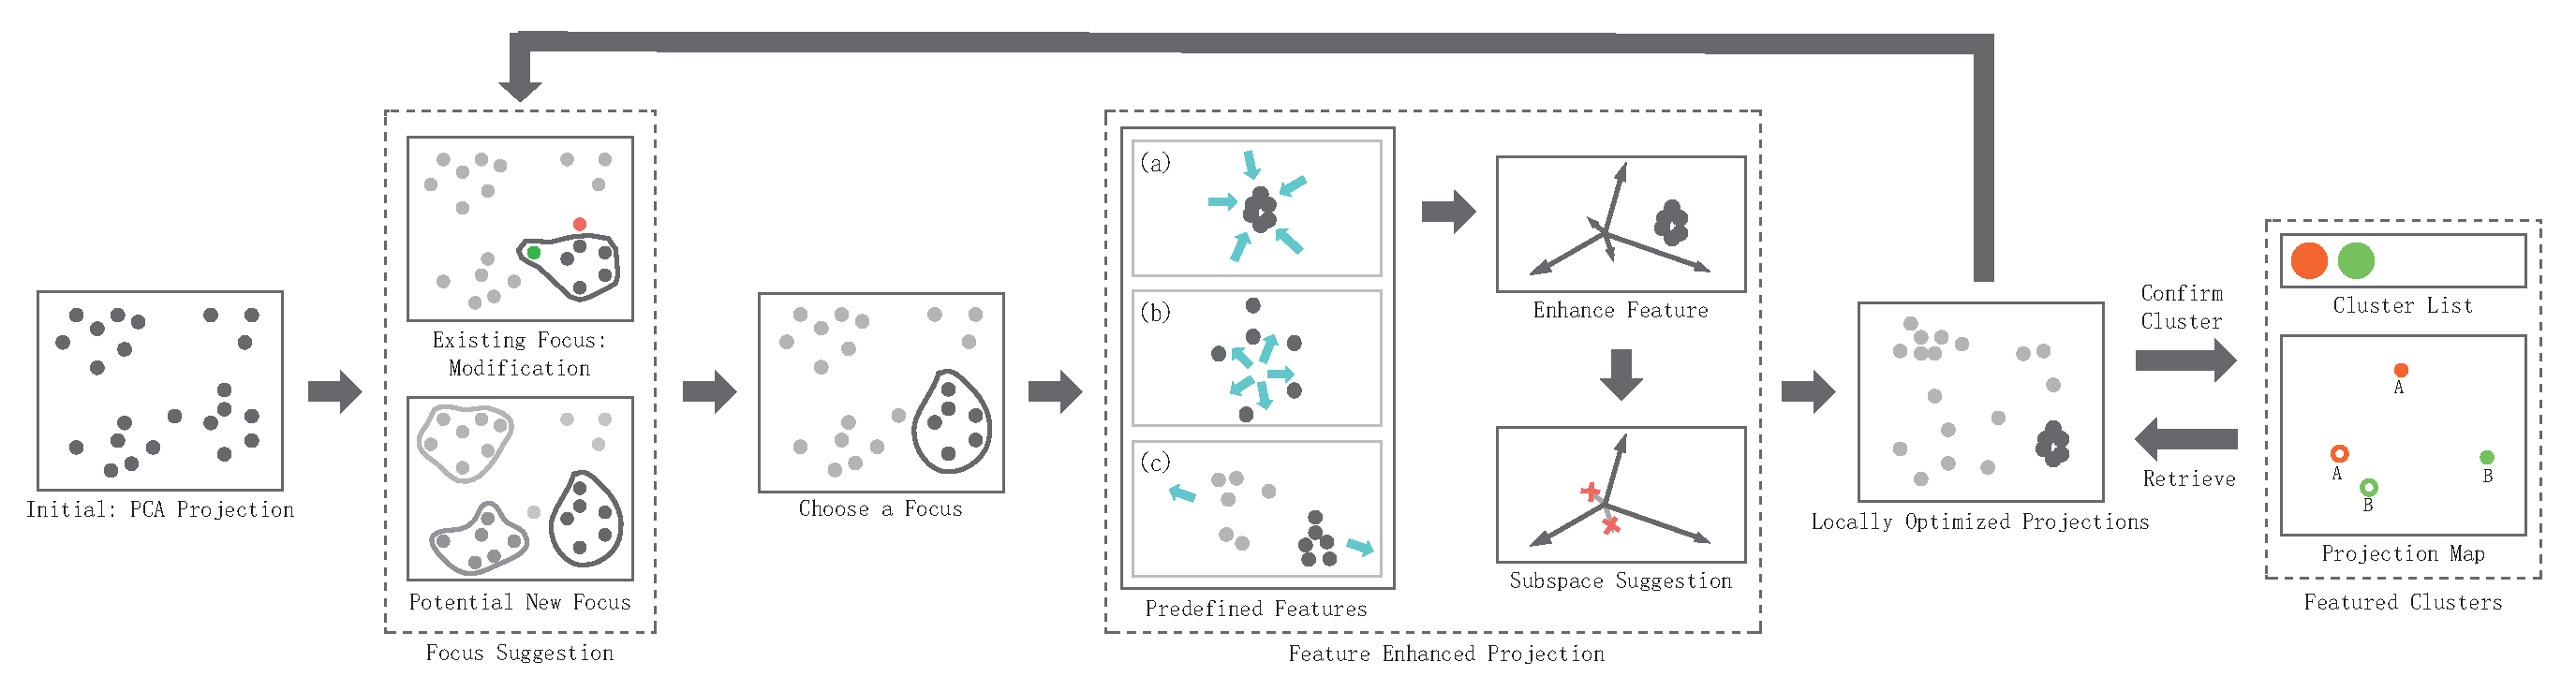
\includegraphics{images/Pipeline.eps}
\caption{Sample illustration.}
\end{figure*}
\else
\begin{figure*}[htbp]
\centering
  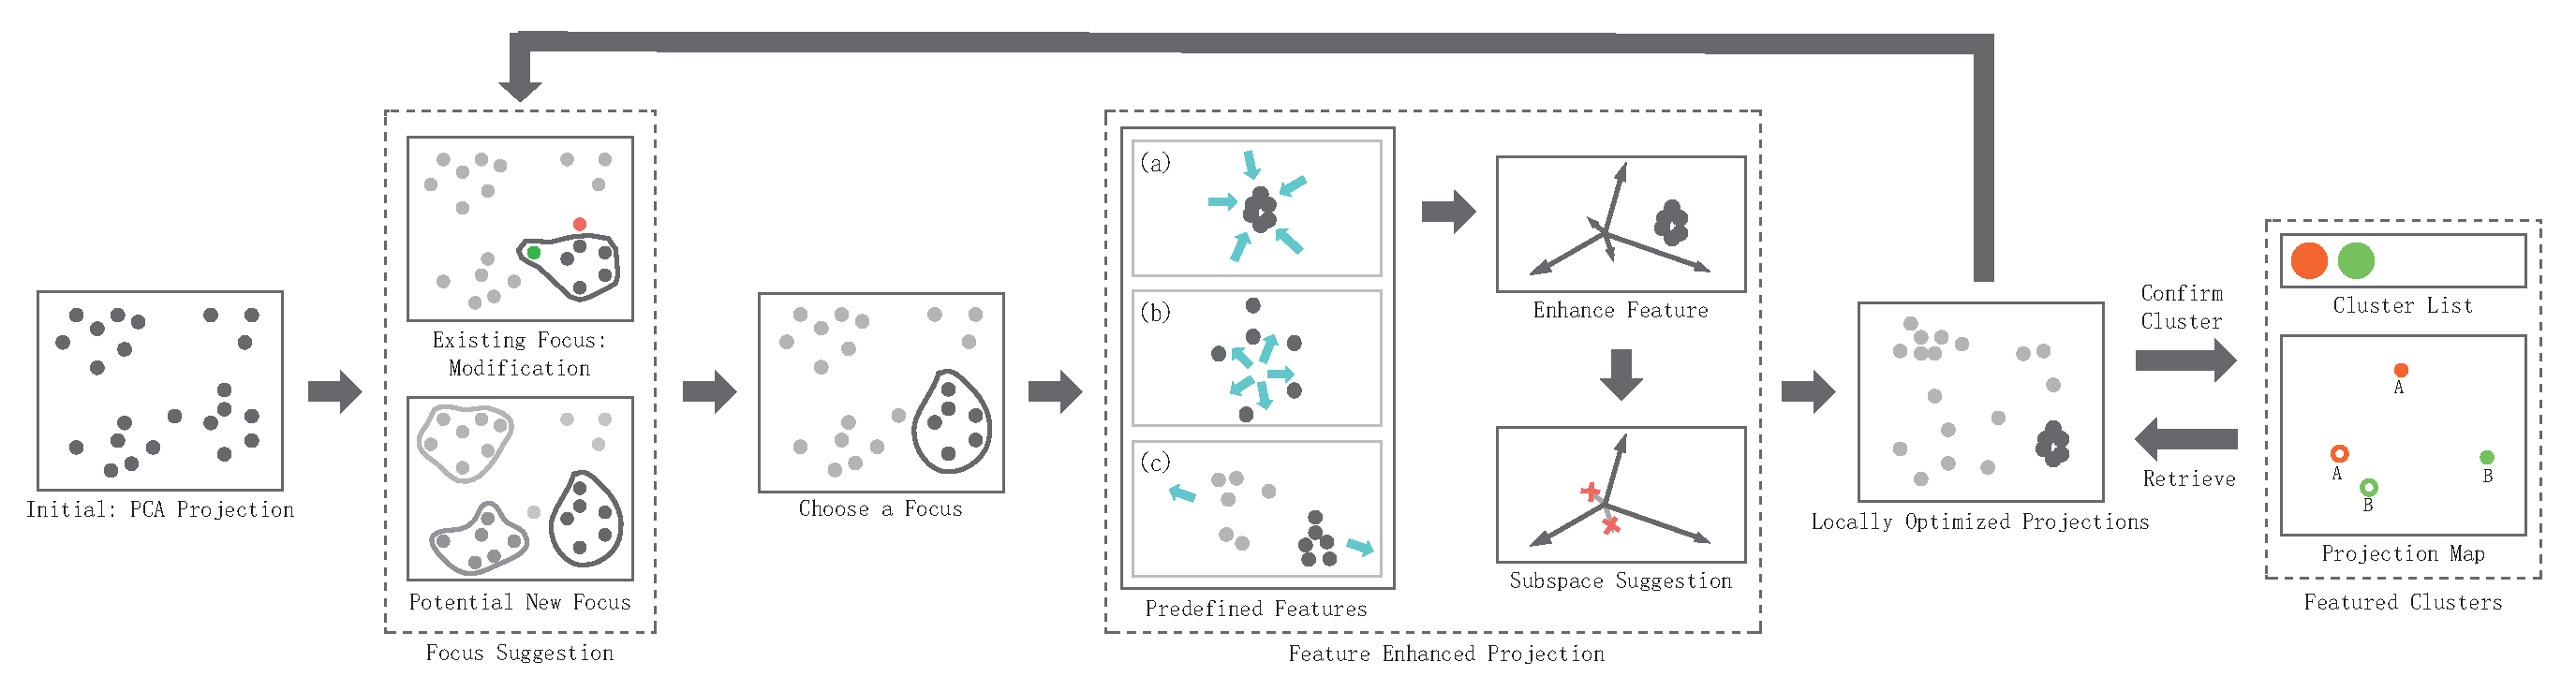
\includegraphics[width=1\linewidth]{images/Pipeline.eps}% 1\linewidth
  \caption{The overview of delivery system.}\label{fig.2}
  \end{figure*}
  \fi